

%%%%%%%%%%%%%%%%%%%%%%%%%%%%%%%%%%%%%%%%%%%%%%%%%%%%%%%%%%%%%%%%%%%%%%%%
% RevTeX 4.1 LaTeX
% Kevin C. Young
% Scalable & Secure Systems Research (08961)
% Thu Mar  5 15:29:19 PST 2015
%%%%%%%%%%%%%%%%%%%%%%%%%%%%%%%%%%%%%%%%%%%%%%%%%%%%%%%%%%%%%%%%%%%%%%%%

\documentclass[aps,nofootinbib,pra,notitlepage,twocolumn]{revtex4-1}

\usepackage{amsfonts,amsmath,amssymb,amsthm}
\usepackage{array,bm,color}
\usepackage{epsfig,graphicx,nomencl,revsymb4-1,upgreek,url}
\usepackage{hyperref}
\usepackage{algorithm}
\usepackage{algpseudocode, caption}
\hypersetup{colorlinks=true, pdfauthor=Kevin C. Young, pdftitle=}
%\hypersetup{citecolor={blue}, colorlinks={true}, filecolor={blue},
%   linkcolor={blue}, pdfauthor=, pdfkeywords= pdfsubject=, pdftitle=,
%   urlcolor{blue}}



\newcommand{\tr}{{\rm Tr\thinspace}}
\newcommand{\bra}[1]{\ensuremath{\left\langle{#1}\right\vert}}
\newcommand{\ket}[1]{\ensuremath{\left\vert{#1}\right\rangle}}
\newcommand{\braket}[2]{\left\langle #1 | #2 \right\rangle}
\newcommand{\ketbra}[2]{\left| #1 \right\rangle\!\!\!\,\left\langle #2 \right|}
\newcommand{\abs}[1]{\left\vert #1 \right\vert}
\newcommand{\expect}[1]{\ensuremath{\left\langle{#1}\right\rangle}}
\newcommand{\timeorder}{\ensuremath{\underset{\leftarrow}{\mathcal{T}}}}
\newcommand{\ident}{{\mathbb1}}
\newcommand{\order}[1]{\mathcal{O}\left( #1 \right)}
\newcommand{\diag}[1]{\mathrm{diag}\{#1\}}
\newcommand{\trans}[1]{#1^\mathsf{T}}
\newcommand{\T}{\mathsf{T}}

\newcommand{\erf}[1]{Eq.~(\ref{#1})}
\newcommand{\needcite}{{\color{blue}\textsuperscript{[citation needed]}}}
\newcommand{\note}[1]{{\color{red}[#1]}}
\newcommand{\kcy}[1]{{\color{red}[#1]_{\rm{KCY}}}}

%-------------Header begins here----------------------------------------
\begin{document}
\title{Decorrelating Errors in Quantum Gates by Random Gate Synthesis}

\author{Kevin C. Young}
\email[Corresponding author: ]{kyoung@sandia.gov}
\affiliation{Sandia National Laboratories, Livermore, CA}

\author{Anthony Polloreno}
% \email[Email: ]{apolloreno}
\affiliation{Rigetti Quantum Computing, Berkeley, CA}

\date{\today}

\begin{abstract}
Thresholds for fault-tolerant quantum computation are often calculated assuming a noise model in which errors are uncorrelated. While convenient for simulation, these error models are often unphysical.  Recent work by Preskill and others has shown that the arbitrarily long computations may be performed even in the presence of spatial correlation, provided the correlation is sufficiently weak and decays sufficiently quickly with distance, but at the cost of a significantly lower threshold. The success of algebraic decorrelation methods, such as dynamical decoupling, demonstrate that quantum control techniques are capable of reducing temporal noise correlations. We propose to introduce similar methods to effect the spatial decorrelation of errors in quantum circuits, thereby increasing the threshold for fault-tolerant computation in such systems.
\end{abstract}

\pacs{}

\maketitle

\section{Outline}
\begin{enumerate}
    \item Introduction
    \item Method
    \item Results
    \item Discussion
    \item Acknowledgments
\end{enumerate}

\section{Introduction}

Thresholds for fault-tolerant quantum computation are often calculated assuming a noise model in which errors are uncorrelated. While convenient for simulation, these error models are often unphysical.  Recent work by Preskill and others has shown that the arbitrarily long computations may be performed even in the presence of spatial correlation, provided the correlation is sufficiently weak and decays sufficiently quickly with distance, but at the cost of a significantly lower threshold. The success of algebraic decorrelation methods, such as dynamical decoupling, demonstrate that quantum control techniques are capable of reducing temporal noise correlations. We propose to introduce similar methods to effect the spatial decorrelation of errors in quantum circuits, thereby increasing the threshold for fault-tolerant computation in such systems.

We propose to inject additional decorrelating randomness into the system through the use of \emph{balanced control solutions} (BCSs).  BCSs are families of control solutions that all approximate the same target gate, but with balanced errors for any given instance of the noise Hamiltonian.  That is, for a target gate, $U_T$, we seek a family of control solutions, $c_i(t)$, each implementing an approximation $U_i$ to the target gate, such that the family of unitary approximations is \emph{balanced}.  A balanced family is one which satisfies, for some small $\alpha$,
\begin{equation}\label{eq:1}
    \frac{1}{N}\sum_{i=1}^N \omega_i U_i \rho U_i^\dagger = DPN[\alpha]\left(U_T \rho U_T^\dagger \right)
\end{equation}

Where $DPN[\alpha](\rho)$ is a depolarizing noise channel with strength $\alpha$. On average, the unitary approximations implement the target unitary followed by a small depolarizing channel. The task of constructing the BCSs will fall to optimal control.



\section{A Simple Example}
As a somewhat trivial example, consider a single-qubit rotation-angle error, such as result from stochastic laser amplitude fluctuations. A BCS may consist of an $X_\pi$ pulse, as well as an $\bar X_\pi$ pulse (ie, a clockwise and counter clockwise rotation of the qubit).  In the case of excess amplitude, the $X_\pi$ pulse will result in an over-rotation error, while the $\bar X_\pi$ pulse results in an \emph{under}-rotation error.  When it comes time to perform the target gate in a quantum circuit, one member of the BCS is chosen uniformly at random.  This has the effect of decorrelating the over-rotation error.  As we show, these techniques may be generalized to multi-qubit errors.


\section{Optimal Control Problem}
Generating BCSs can be done in a variety of ways. For simplicity in this paper we use the GRAPE algorithm to generate candidate pulseshapes to approximate the target gate, but one could use any quantum optimal control technique find a family of controls. In our numerical experiment, we set our target control infidelity to $\epsilon=1\mathrm{e}{-3}$ and model the stochastic error on the controls as normally distributed random variables, so that each time-varying control $c_i(t)$ has an associated error $\delta_i \mathtt{\sim} \mathcal{N}(0, .001)$
Thus we have the following Hamiltonian:
\begin{equation}\label{eq:2}
  H(t) = H_0 + \sum_{i=0}^n (c_i(t) + \delta_i)H_i
\end{equation}
for control Hamiltonians $H_i$ and free evolution Hamiltonian $H_0$. In the update step for GRAPE, we modify the gradient to be that of the weighted average performance, with the integrals approximated via Gaussian quadrature:
\begin{equation}
   \mathcal{T}[\int p(\vec{\delta})e^{-iH(t)t}dtd\vec{\delta}]\\
\end{equation}
where $p(\vec{\delta})$ is a multivariate Gaussian distribution.
Doing this ensures that our family of controls perform moderately well over a range of stochastic errors.

After using GRAPE to produce a collection of controls, we now must find the weights $w_i$ such that the collection of controls form a BCS as described in (\ref{eq:1}). To do this, for each control $U_i$ we find the unitary error channel $\mathcal{E}_i$ such that $\mathcal{E}_iU_i=U_T$, where $U_T$ is the target gate. If we consider the Pauli-Liouville representation of this error channel, the diagonal terms are the \textit{stochastic} terms that arise from classical uncertainty, while the off-diagonal terms may more generally arise from \textit{coherent} operations. In particular, we see that we can write a convex sum over these channels as:
\begin{align}
 \frac{1}{N} \sum^N_{i=1} w_i \mathcal{E}^{\dagger} (U_T\rho U_T^{\dagger}) \mathcal{E}
\end{align}
Now, to approximate a depolarizing channel we define our optimal control problem to be the following, which minimizes the off-diagonal terms:
\begin{align}
   &\underset{w_0, ..., w_N}{\textbf{minimize}} \{\sum_{i\neq j}^N|\sigma_i\Lambda(\sigma_j)|^2\}\\
   &\textbf{where}\ \Lambda(\sigma_j) := \sum^N_{i=1}w_i\mathcal{E}_i^{\dagger}\sigma_j\mathcal{E}_i\\
   &\textbf{subject to} \sum_{i=1}^Nw_i = 1
\end{align}

This can be solved with a constrained minimization algorithm, such as Sequential Least Squares Programming. We present numerical results for one qubit and two qubits gates in the following sections.

\section{GRAPE}
First described in \cite{Khaneja2005}, the GRAPE (GRadient Ascent Pulse Engineering) algorithm is a technique for finding piecewise constant control sequences that approximate a desired unitary. Naively this can be done by defining a cost function $J(U) = Tr\{U_TU\}$, where $U_T$ is the target unitary, and $U = \exp\{-it(H_0 + \sum_{i=0}^{n}(c_i(t)H_i)\}$. One can then define the \textit{control matrix} $u_{ij}$, denoting the control amplitude associated with the $i^{th}$ time step and the $j^{th}$ hamiltonian. Then we see that we can maximize our cost function via the chain rule, i.e. performing the following update loop for some threshold value $\delta$:

\begin{algorithm}[H]
\floatname{algorithm}{Procedure}
  \caption*{\textsc{\textbf{Gradient Ascent}}}
   \begin{algorithmic}
\While{$J(U) < (1-\delta$)}
\State $u_{ij}$ $\rightarrow$ $u_{ij} + \epsilon\frac{\partial J(U)}{\partial u_{ij}}$
\State $U \rightarrow \exp\{-it(H_0 + \sum_{i=0}^{n}(c_i(t)H_i)\}$
\EndWhile

   \end{algorithmic}
\end{algorithm}


In general these gradients can be computed by propagating partial derivatives of the cost function with respect to control parameters via the chain rule. However, in \cite{Khaneja2005} Khaneja et al. derive a simple update formula that is correct to first order, in particular one can show that:
\begin{align}
\frac{\partial J(U)}{\partial u_{ij}} = -2Re\{\braket{{U_{j+1}^{\dagger}...U_N^{\dagger} U_T}}{i\Delta tH_jU_j...U_1}\\
\braket{U_j...U_1}{U_{j+1}^{\dagger}...U_N^{\dagger} U_T}\} +  \mathcal{O}(\Delta t^2)
\end{align}

In this paper we have modified the update step to use instead use approximately the following gradient:
\begin{align}
\int p(\vec{\delta})\frac{\partial J(U(\vec{\delta})}{\partial u_{ij}} d\vec{\delta}
\end{align}
again with $p(\vec{\delta})$ Gaussian. In particular, this ensures that the optimizer will attempt to find controls that are not only good at zero detuning, but also for small noise values.
\begin{figure*}
\centering
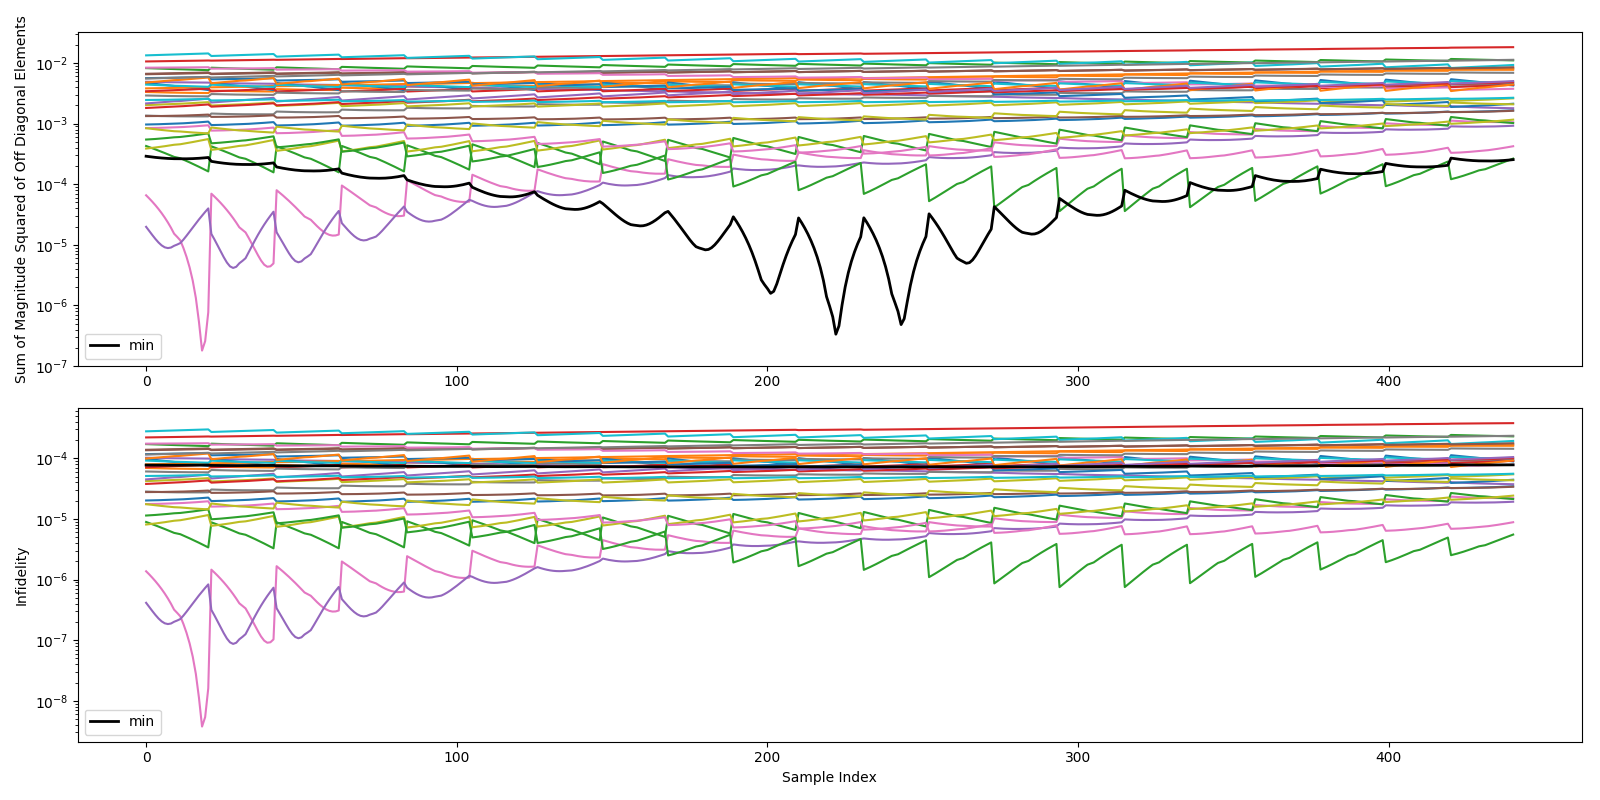
\includegraphics[width=\textwidth]{x2.png}
\caption{In the above we have used our method to produce a BCS for a $RX(\frac{\pi}{2})$ pulse, with the Hamiltonian given in \ref{eq:1Qham}. A) shows the sum of the squared norms of the off diagonal terms in the Pauli Transfer Matrix of $\mathcal{E}$. B) gives the corresponding infidelity for each member of the BCS, and the optimal choice of weights.}
\end{figure*}
\begin{figure*}
\centering
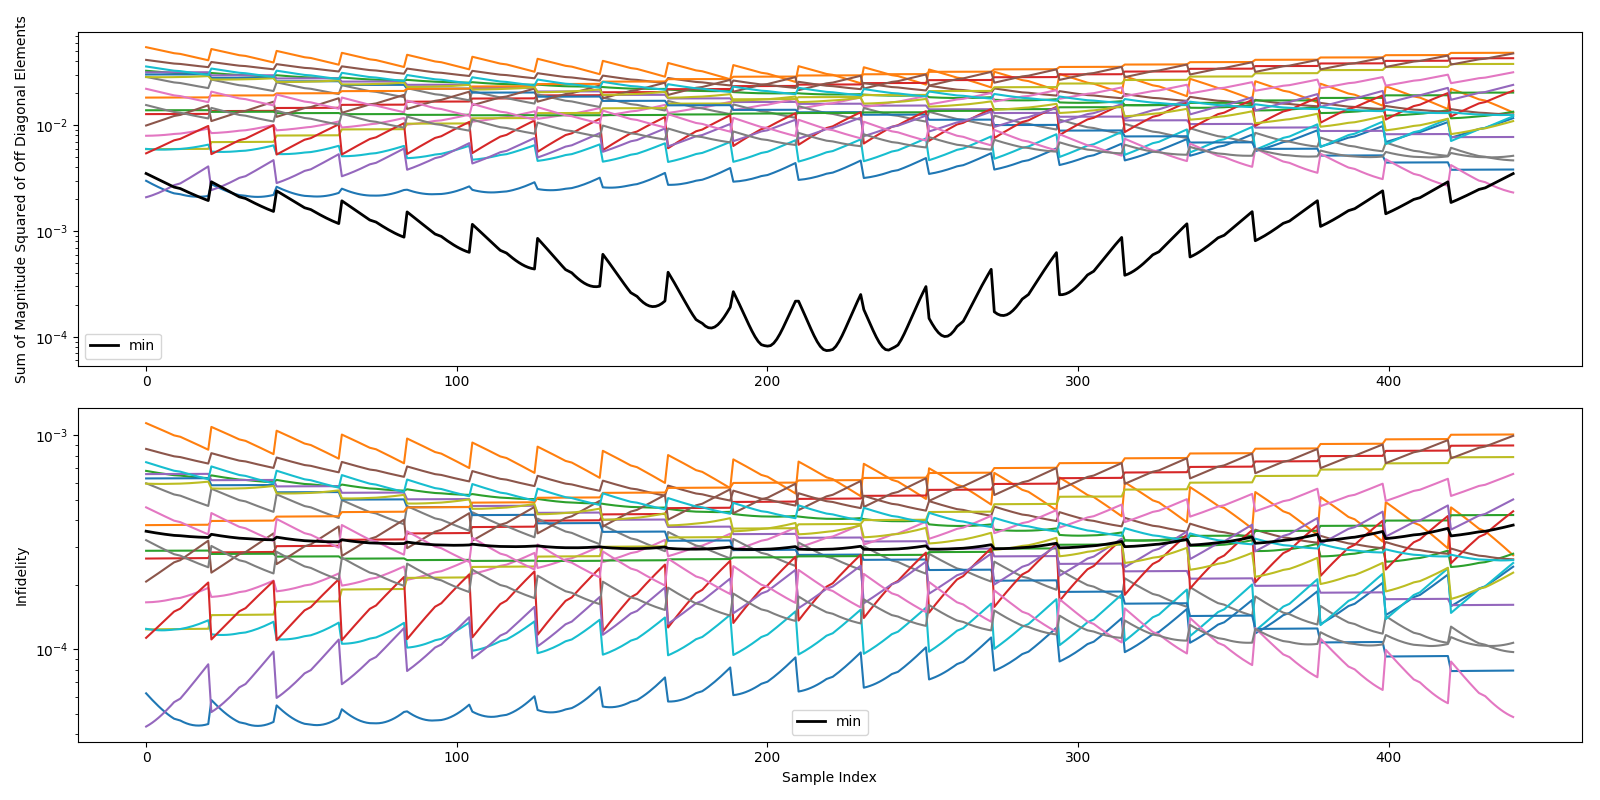
\includegraphics[width=\textwidth]{y2.png}
\caption{In the above we have used our method to produce a BCS for a $RY(\frac{\pi}{2})$ pulse, with the Hamiltonian given in \ref{eq:1Qham}. A) shows the sum of the squared norms of the off diagonal terms in the Pauli Transfer Matrix of $\mathcal{E}$. B) gives the corresponding infidelity for each member of the BCS, and the optimal choice of weights.}
\end{figure*}

\section{1Q Gates}
We assume a model of our Hamiltonian for one qubit control to be:

\begin{equation}\label{eq:1Qham}
H = \epsilon\sigma_z + (1 + \delta)(c_x(t)\sigma_x + c_y(t)\sigma_y)
\end{equation}
We assume variances of $\sigma = .001$ on all control parameters, and we use a control time of $\pi$, with 100 steps of discretization. We assume that the errors on $\sigma_x$ and $\sigma_y$ are perfecly correlated.
%These plots take a little while to make, so I can't iterate *that* fast - clearly the fonts need to be bigger, and there should be a title what else add a legend saying the black is the optimal?
\begin{figure*}
\centering
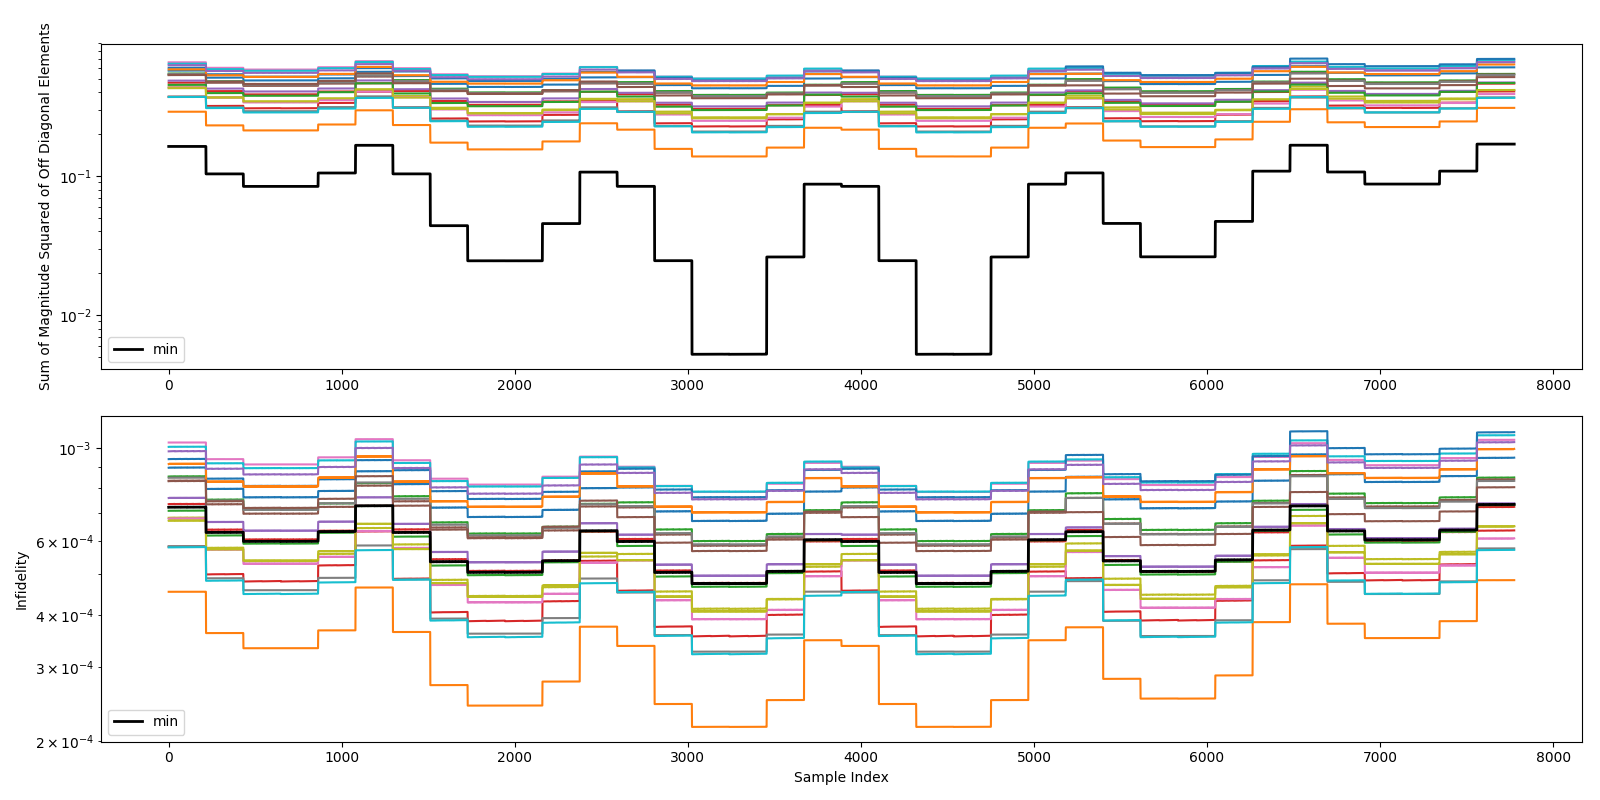
\includegraphics[width=\textwidth]{2Q.png}
\caption{In the above we have used our method to produce a BCS for a ZZ($\frac{\pi}{2}$) entangling gate with controls given by \ref{eq:2Qham}. A) shows the sum of the squared norms of the off diagonal terms in the Pauli Transfer Matrix of $\mathcal{E}$. B) gives the corresponding infidelity for each member of the BCS, and the optimal choice of weights.}
\end{figure*}

\section{2Q Gate}
We assume a model of our Hamiltonian for two qubit control to be:
\begin{equation} \label{eq:2Qham}
H = \sum_{j=1}^2\epsilon_j\sigma_z^j + (1 + \delta_j)(c_x^jx(t)\sigma_x^j + c_y^j(t)\sigma_y^j)
\end{equation}
We assume that the standard deviations are $\sigma = .001$ on all parameters, and that the control time is 4 $\pi$, with discretization of 500 steps. In addition, we assume that errors on the single qubit $\sigma_x$ and $\sigma_y$ rotations are correlated. Namely, because in many systems like superconducting qubits, the difference between these pulses amounts to a phase shift in the signal, so that things like amplitude drift will be shared and correlated.
%It might be interesting to show a dhistogram of the pribabilities assigned to each control to show that they aren't all zero. and maybe 



%$$ \epsilon, \delta \midtilde \sim \mathcal{N}(0, .001) $$
%$$\epsilon_0, \epsilon_1, \delta_0, \delta_1 \midtilde \sim \mathcal{N}(0, .001)$$
\bibliography{decorrelation.bib}
\end{document}
